% fs-09-hyptest.tex

\documentclass[xcolor=dvipsnames]{beamer}

\usepackage{tikz}
\usepackage{graphicx}
\usepackage{wrapfig}
\usepackage{colortbl}
\usepackage{alltt}
\definecolor{myblue}{rgb}{0.8,0.85,1}

\mode<presentation>
{
  \usetheme{Warsaw}
  \setbeamercovered{transparent}
}
% \usecolortheme[named=OliveGreen]{structure}
\setbeamertemplate{navigation symbols}{} 
\setbeamertemplate{blocks}[rounded][shadow=true] 

\newcounter{expls}
\setcounter{expls}{0}
\newcommand{\beispiel}[1]{\refstepcounter{expls}\textbf{Example \arabic{expls}: #1.}}

\newcounter{exercise}
\setcounter{exercise}{0}
\newcommand{\ubung}[0]{\refstepcounter{exercise}\textbf{Exercise \arabic{exercise}: }}

\makeatletter
\newcommand\binomialCoefficient[2]{%
    % Store values 
    \c@pgf@counta=#1% n
    \c@pgf@countb=#2% k
    %
    % Take advantage of symmetry if k > n - k
    \c@pgf@countc=\c@pgf@counta%
    \advance\c@pgf@countc by-\c@pgf@countb%
    \ifnum\c@pgf@countb>\c@pgf@countc%
        \c@pgf@countb=\c@pgf@countc%
    \fi%
    %
    % Recursively compute the coefficients
    \c@pgf@countc=1% will hold the result
    \c@pgf@countd=0% counter
    \pgfmathloop% c -> c*(n-i)/(i+1) for i=0,...,k-1
        \ifnum\c@pgf@countd<\c@pgf@countb%
        \multiply\c@pgf@countc by\c@pgf@counta%
        \advance\c@pgf@counta by-1%
        \advance\c@pgf@countd by1%
        \divide\c@pgf@countc by\c@pgf@countd%
    \repeatpgfmathloop%
    \the\c@pgf@countc%
}
\makeatother

\newif\ifBCITCourse
\BCITCoursetrue
% \BCITCoursefalse
\newif\ifWhichCourse
\WhichCoursetrue
% \WhichCoursefalse
\ifBCITCourse
\ifWhichCourse
\newcommand{\CourseName}{Statistics for Food Technology}
\newcommand{\CourseNumber}{MATH 2441}
\newcommand{\CourseInst}{BCIT}
\else
\newcommand{\CourseName}{Calculus for Geomatics}
\newcommand{\CourseNumber}{MATH 2511}
\newcommand{\CourseInst}{BCIT}
\fi
\else
\newcommand{\CourseName}{Philosophy and Literature}
\newcommand{\CourseNumber}{PHIL 375}
\newcommand{\CourseInst}{UBC}
\fi

\newcommand{\puw}{9}
\newcommand{\iex}{13}
\newcommand{\nae}{40}
\newcommand{\mih}{3}
\newcommand{\esh}{91.1}
\newcommand{\chu}{5.8}
\newcommand{\pee}{735}
\newcommand{\ood}{19.2}
\newcommand{\tee}{78.3}
\newcommand{\aih}{600}
\newcommand{\aoj}{20}
\newcommand{\eep}{140}
\newcommand{\eim}{12}
\newcommand{\sho}{90}

\title{Hypothesis Testing}
\subtitle{{\CourseNumber}, BCIT}

\author{\CourseName}

\date{March 30, 2017}

% \begin{figure}[h]
% 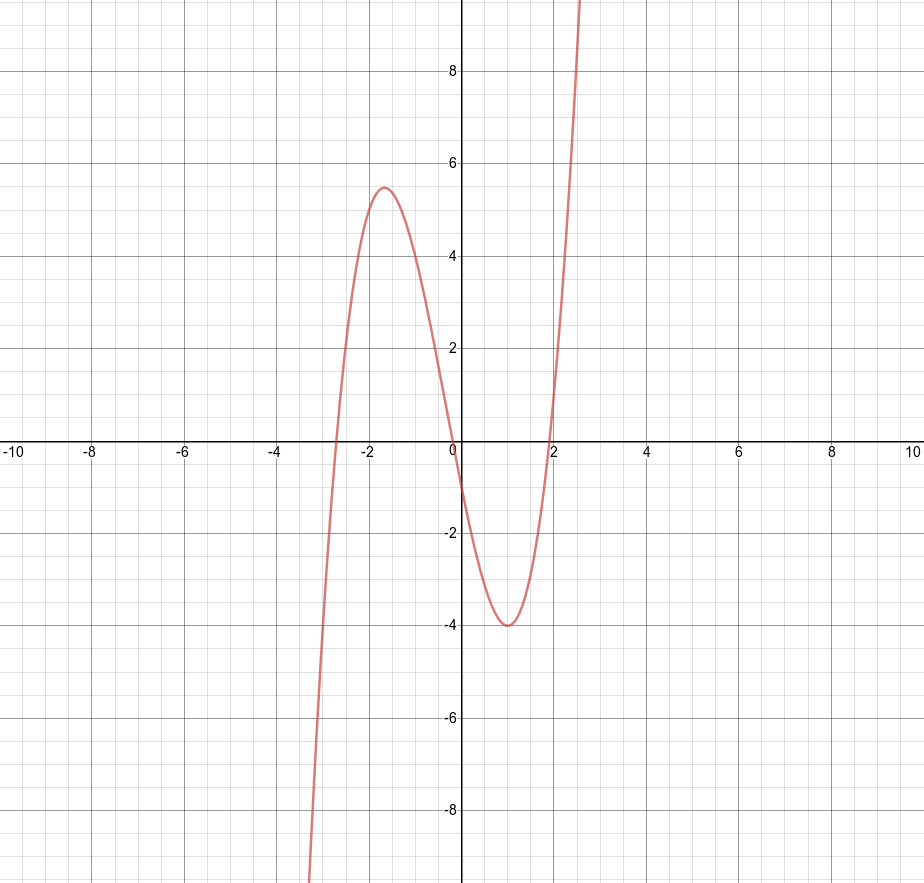
\includegraphics[scale=.3]{./diagrams/extrema1.png}
% \end{figure}

% Command             10pt    11pt    12pt
% \tiny               5       6       6
% \scriptsize         7       8       8
% \footnotesize       8       9       10
% \small              9       10      10.95
% \normalsize         10      10.95   12

\begin{document}

\begin{frame}
  \titlepage
\end{frame}

\begin{frame}
  \frametitle{Hypothesis Testing}
  What we have done so far is to make an inference about a statistic
  (proportion, mean, variance) based on a sample. Often, however,
  the method of science requires the reverse procedure: articulate a
  hypothesis and then test it to see if you can falsify it. For
  example, there may be a new medical treatment available or a new
  method of conserving a certain food item. A scientist then wants to
  test if the new method makes a difference compared to the old
  method. This is why for our next topic we will address what
  inferences we can make on the basis of two samples. First, we have
  to reverse our procedure and sort out what it means to articulate a
  hypothesis and then test it.
\end{frame}

\begin{frame}
  \frametitle{Concepts of Hyothesis Testing}
  \begin{description}
  \item[Null Hypothesis] The null hypothesis is the statement that the
    value of a population parameter (such as a proportion, a mean, or
    a variance) is equal to some claimed value. Example: $p=0.5$.
    Decision: \alert{reject} or \alert{fail to reject}.
  \item[Alternative Hypothesis] The alternative hypothesis states that
    the null hypothesis is false. Examples: $p>0.5$ or $p<0.5$ or
    $p\neq{}0.5$. Decision: \alert{accept} or
    \alert{fail to accept}.
  \item[Test Statistic] The test statistic is a value used in making a
    decision about the null hypothesis. It is found by converting the
    sample statistic (the sample proportion $\hat{p}$, the sample mean
    $\bar{x}$, or the sample standard devises $s$) to a score (such as
    $z$, $t$, or $\chi^{2}$) with the assumption that the null
    hypothesis is true.
  \end{description}
\end{frame}

\begin{frame}
  \frametitle{Test Statistic Table}
  \begin{figure}[h]
    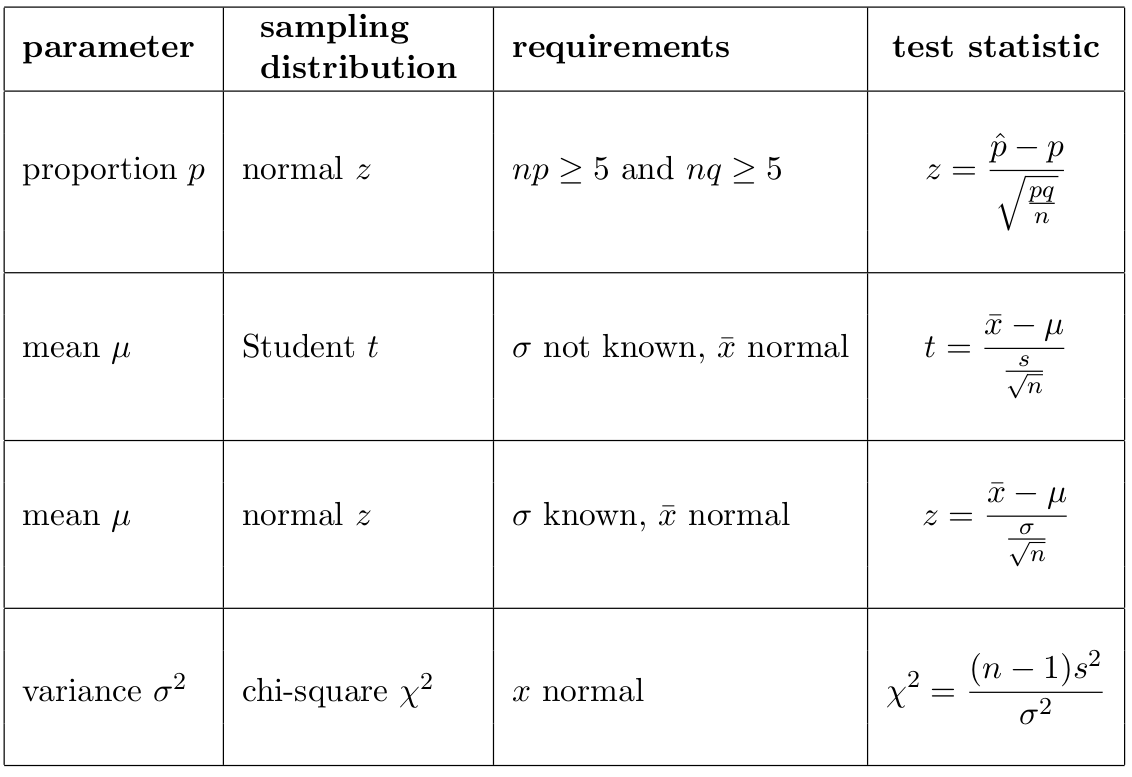
\includegraphics[scale=0.27]{./diagrams/hyptesttab.png}
  \end{figure}
% the following was latexed in siri and shuttered
%   \begin{tabular}{|l|l|l|c|}\hline
%     \textbf{parameter} & \begin{tabular}{l} \textbf{sampling} \\ \textbf{distribution} \end{tabular} & \textbf{requirements} & \textbf{test statistic} \\ \hline
% \hspace{.5in} & \hspace{.5in} & \hspace{.5in} & \hspace{.5in} \\ 
%     proportion $p$     & normal $z$            & $np\geq{}5$ and $nq\geq{}5$ & $\displaystyle z=\frac{\hat{p}-p}{\sqrt{\frac{pq}{n}}}$ \\
% \hspace{.5in} & \hspace{.5in} & \hspace{.5in} & \hspace{.5in} \\ \hline
% \hspace{.5in} & \hspace{.5in} & \hspace{.5in} & \hspace{.5in} \\
%     mean $\mu$         & Student $t$           & $\sigma$ not known, $\bar{x}$ normal &  $\displaystyle t=\frac{\bar{x}-\mu}{\frac{s}{\sqrt{n}}}$ \\
% \hspace{.5in} & \hspace{.5in} & \hspace{.5in} & \hspace{.5in} \\ \hline
% \hspace{.5in} & \hspace{.5in} & \hspace{.5in} & \hspace{.5in} \\
%     mean $\mu$         & normal $z$           & $\sigma$ known, $\bar{x}$ normal &  $\displaystyle z=\frac{\bar{x}-\mu}{\frac{\sigma}{\sqrt{n}}}$ \\
% \hspace{.5in} & \hspace{.5in} & \hspace{.5in} & \hspace{.5in} \\ \hline
% \hspace{.5in} & \hspace{.5in} & \hspace{.5in} & \hspace{.5in} \\
%     variance $\sigma^{2}$         & chi-square $\chi^{2}$           & $x$ normal &  $\displaystyle \chi^{2}=\frac{(n-1)s^{2}}{\sigma^{2}}$ \\
% \hspace{.5in} & \hspace{.5in} & \hspace{.5in} & \hspace{.5in} \\ \hline
%   \end{tabular}
\end{frame}

\begin{frame}
  \frametitle{Examples I}
  \begin{description}
  \item[Law] Republicans claimed in a lawsuit that a New Jersey county
    clerk did not use a required method of random selection when he
    chose a Democratic cadidate to be first on the ballot in 40 out of
    41 elections.
  \item[Genetics] The Genetics \& IVF Institute claims that its XSORT
    method allows couples to increase the probability of having a baby
    girl, and sample evidence consists of 879 girls among 945 couples
    treated with the XSORT method.
  \item[Health] It is often claimed that the mean body temperature is
    $98.6^{\circ}$F, and we can test that claim using the data
    provided earlier, which includes a sample of 106 body temperatures
    with a mean of $98.2^{\circ}$F.
  \end{description}
\end{frame}

\begin{frame}
  \frametitle{Examples II}
  \begin{description}
  \item[Business] A newspaper cites a \texttt{PriceGrabber.com} survey
    of 1631 subjects and claims that the majority of consumers have
    heard of the Kindle as an e-book reader.
  \item[Quality Control] When new equipment is used to manufacture
    temperature gauges for the food industry, the new gauges are
    better because the variation in the errors is reduced so that the
    readings are more consistent. In many industries, the quality of
    goods and services can often be improved by reducing variation.
  \end{description}
\end{frame}

\begin{frame}
  \frametitle{Hypothesis Testing: Procedure}
  \begin{description}
  \item[Step 1] Identify the null and the alternative hypothesis in
    symbolic form.
  \item[Step 2] Identify the statistic that is relevant to this test
    and determine its sampling distribution (normal, Student $t$, or
    chi-square).
  \item[Step 3] Use the $p$-value method or the critical value method
    to reject the null hypothesis or to fail to reject the null
    hypothesis.
  \end{description}
\end{frame}

\begin{frame}
  \frametitle{Hypothesis Testing: Procedure}
  \begin{figure}[h]
    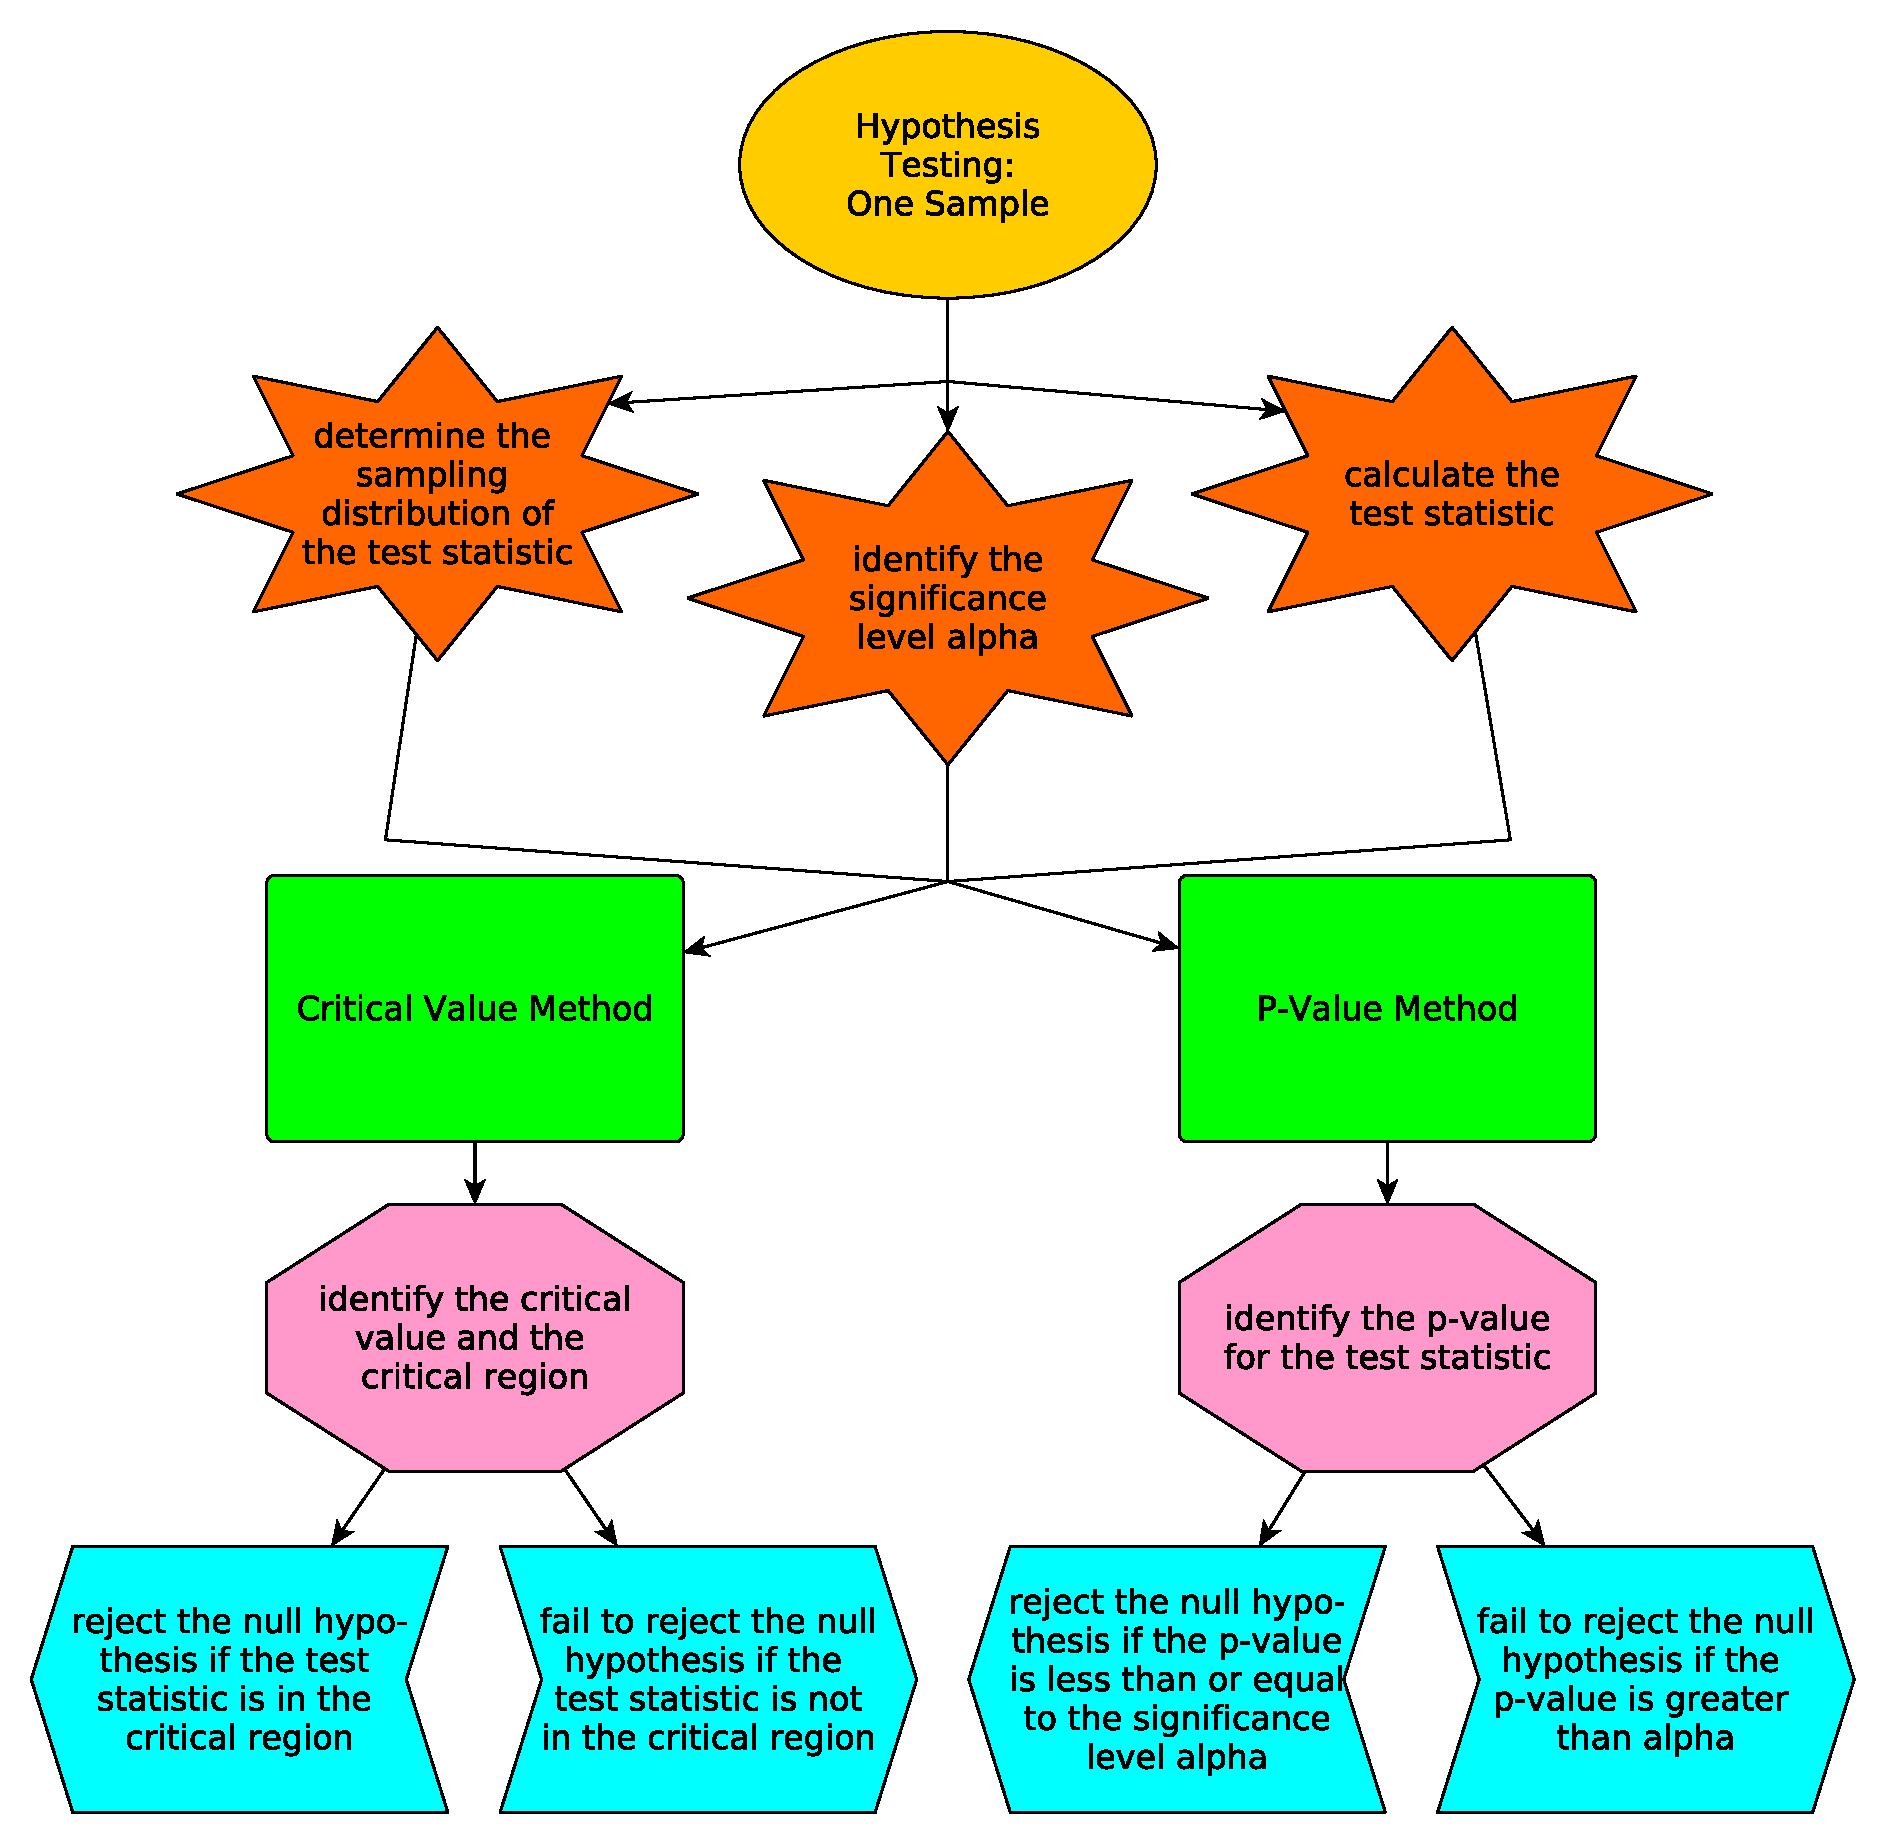
\includegraphics[scale=0.25]{./diagrams/hypoONEsample.pdf}
  \end{figure}
\end{frame}

\begin{frame}
  \frametitle{Hypothesis Testing: Proportion}
  \beispiel{Gender XSORT Method} The Genetics \& IVF Institute claims
  that its XSORT method allows couples to increase the probability of
  having a baby girl, and sample evidence consists of 879 girls among
  945 couples treated with the XSORT method.

  The null hypothesis is ``the XSORT method makes no difference,''
  $p=0.5$; the alternative hypothesis is ``the XSORT method makes a
  difference and favours the birth of girls,'' $p>0.5$. This is a
  \alert{right-tailed test} (as opposed to a \alert{left-tailed test}
  or a \alert{two-tailed test}). Let's set the significance level at
  $1-\alpha=0.95$.

The test statistic for proportions is 
\begin{equation}
  \label{eq:bahhixie}
  z=\frac{\hat{p}-p}{\sqrt{\frac{pq}{n}}}=\frac{\frac{879}{945}-\frac{1}{2}}{\sqrt{\frac{\frac{879}{945}\cdot\frac{66}{945}}{945}}}=51.881
\end{equation}
\end{frame}

\begin{frame}
  \frametitle{Hypothesis Testing: Proportion}
The test statistic for proportions is 
\begin{equation}
  \label{eq:aegaasee}
  z=\frac{\hat{p}-p}{\sqrt{\frac{pq}{n}}}=\frac{\frac{879}{945}-\frac{1}{2}}{\sqrt{\frac{\frac{879}{945}\cdot\frac{66}{945}}{945}}}=51.881
\end{equation}

You can see that this result is beyond the pale. There is (just about)
no way that 879 out of 945 births are girls if the true proportion for
the population is $p=0.5$. We reject the null hypothesis because
\begin{description}
\item[$p$-value method] $0.05\geq{}0+$, where $0+$ is the $p$-value for
  $z=51.881$.
\item[critical value method] $51.881\geq{}1.645$, where $1.645$ is the
  critical value for a significance level of $1-\alpha=0.95$ and a
  right-tailed test.
\end{description}
\end{frame}

\begin{frame}
  \frametitle{Type I and Type II Error}
  \begin{figure}[h]
    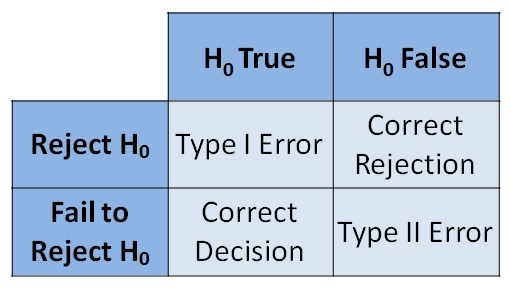
\includegraphics[scale=0.5]{./diagrams/error.jpg}
  \end{figure}
\end{frame}

\begin{frame}
  \frametitle{Hypothesis Testing: Proportion}
  {\ubung} You buy a bag of M\&Ms. The bag contains 100 M\&Ms, eight
  of which are brown. Use a $0.05$ significance level to test the
  claim of the Mars candy company that the percentage of brown M\&Ms
  is equal to 13\%.
\end{frame}

\begin{frame}
  \frametitle{Hypothesis Testing: Proportion}
  {\ubung} In a poll, 806 adults were asked to identify their favourite seat
  when they fly, and 492 of them chose a window seat. Use a $0.01$
  significance level to test the claim that the majority of adults
  prefer window seats when they fly.
\end{frame}

\begin{frame}
  \frametitle{Hypothesis Testing: Proportion}
  {\ubung} In a research poll, 1002 adults were asked if they felt
  vulnerable to identity theft, and 531 of them said ``yes.'' Use a
  $0.05$ significance level to test the claim that the majority of
  adults feel vulnerable to identity theft.
\end{frame}

\begin{frame}
  \frametitle{Hypothesis Testing: Proportion} 
  {\ubung} The Pew Research Center conducted a survey of 1007 adults
  and found that 856 of them know what Twitter is. Use a 0.01
  significance level to test the claim that more than 75\% of adults
  know what Twitter is.
\end{frame}

\begin{frame}
  \frametitle{Hypothesis Testing: Proportion}
  {\ubung} In ``The Overtime Rule in the National Football League:
  Fair or Unfair?'' the authors report that among 414 football games
  won in overtime, 235 were won by the team that won the coin toss at
  the beginning of overtime. Using a 0.05 significance level, test the
  claim that the coin toss is fair in the sense that neither team has
  an advantage by winning it.
\end{frame}

\begin{frame}
  \frametitle{Hypothesis Testing: Proportion}
  {\ubung} In one study of smokers who tried to quit smoking with
  nicotine patch therapy, 39 were smoking one year after the treatment
  and 32 were not smoking one year after the treatment. Use a 0.05
  significance level to test the claim that among smokers who try to
  quit with nicotine patch therapy, the majority are smoking a year
  after the treatment. What do these results suggest about the
  effectiveness of nicotine patch therapy for those trying to quit
  smoking?
\end{frame}

\begin{frame}
  \frametitle{Hypothesis Testing: Proportion}
  {\ubung} A survey of 380 smartphone users showed that 152 of them
  said that their smartphone is the only thing they could not live
  without. Use a 0.01 significance level to test the claim that fewer
  than half of smartphone users identify the smartphone as the only
  thing they could not live without. Do these results apply to the
  general population?
\end{frame}

\begin{frame}
  \frametitle{Hypothesis Testing: Proportion}
  {\ubung} An interesting and popular hypothesis is that individuals
  can temporarily postpone death to survive a major holiday or
  important event such as a birthday. In a study of this phenomenon,
  it was found that there were 6062 deaths in the week before
  Thanksgiving, and 5938 deaths the week after Thanksgiving (based on
  data from ``Holidays, Birthdays, and Postponement of Cancer Death.''
  by Young and Hade, Journal of the American Medical Association,
  Vol.\ 292, No.\ 24). If people can postpone death until after
  Thanksgiving, then the proportion of deaths in the week before
  should be less chan 0.5. Use a 0.05 significance level to test the
  claim that the proportion of deaths in the week before Thanksgiving
  is less than 0.5. Based on the result, does there appear to be any
  indication that people can temporarily postpone death to survive the
  Thanksgiving holiday?
\end{frame}

\begin{frame}
  \frametitle{Hypothesis Testing: Proportion}
  {\ubung} A Consumer Reports Research Center survey of 427 women
  showed that 29.0\% of them purchase books online. Test the
  claim that more than 25\% of women purchase books online.
\end{frame}

\begin{frame}
  \frametitle{Hypothesis Testing: Proportion}
  {\ubung} In a Harris poll of 514 human resource professionals,
  45.9\% said that body piercings and tattoos were big
  grooming red flags. Use a 0.01 significance level to test the claim
  that less than half of all human resource professionals say that
  body piercings are big grooming red flags.
\end{frame}

\begin{frame}
  \frametitle{Hypothesis Testing: Proportion}
  {\ubung} In a Harris poll of 514 human resource professionals, 90\%
  said that the appearance of a job applicant is most important for a
  good first impression. Use a 0.01 significance level to test the
  claim that more than 3/4 of all human resource professionals say
  that the appearance of a job applicant is most important for a good
  first impression.
\end{frame}

\begin{frame}
  \frametitle{Hypothesis Testing: Proportion}
  {\ubung} Voting records show that 61\% of eligible voters actually
  did vote in a recent presidential election. In a survey of 1002
  people, 70\% said that they voted in that election (based on data
  from ICR Research Group). Use the survey results to test the claim
  that the percentage of all voters who say that they voted is equal
  to 61\%. What do the results suggest?
\end{frame}

\begin{frame}
  \frametitle{Hypothesis Testing: Mean}
  {\ubung} The next slide lists ages of actresses when
  they won Oscars, and the summary statistics are
  $n=82,x=35.9,s=11.1$ with years being the unit. Use a
  0.01 significance level to test the claim that the
  mean age of actresses when they win Oscars is 33
  years.
\end{frame}

\begin{frame}[fragile]
  \frametitle{Oscar Actresses Data}
\begin{verbatim}
+--+--+--+--+--+--+--+--+--+--+--+--+--+--+--+--+--+--+
|22|37|28|63|32|26|31|27|27|28|30|26|29|24|38|25|29|41|
+--+--+--+--+--+--+--+--+--+--+--+--+--+--+--+--+--+--+
|30|35|35|33|29|38|54|24|25|46|41|28|40|39|29|27|31|38|
+--+--+--+--+--+--+--+--+--+--+--+--+--+--+--+--+--+--+
|29|25|35|60|43|35|34|34|27|37|42|41|36|32|41|33|31|74|
+--+--+--+--+--+--+--+--+--+--+--+--+--+--+--+--+--+--+
|33|50|38|61|21|41|26|80|42|29|33|35|45|49|39|34|26|25|
+--+--+--+--+--+--+--+--+--+--+--+--+--+--+--+--+--+--+
|33|35|35|28|30|29|61|32|33|45|  |  |  |  |  |  |  |  |
+--+--+--+--+--+--+--+--+--+--+--+--+--+--+--+--+--+--+
\end{verbatim}
\end{frame}

\begin{frame}
  \frametitle{Hypothesis Testing: Mean}
  {\ubung} The weights (lb) of discarded plastic from a
  sample of households is listed on the next slide, and
  the summary statistics are $n=62,x=1.911,s=1.065$.
  Use a 0.05 significance level to test the claim that
  the mean weight of discarded plastic from the
  population of households is greater than 1.800 lb.
\end{frame}

\begin{frame}[fragile]
  \frametitle{Plastic Garbage Data}
\begin{verbatim}
+----+----+----+----+----+----+----+----+----+----+
|0.27|1.41|2.19|2.83|2.19|1.81|0.85|3.05|3.42|2.10|
+----+----+----+----+----+----+----+----+----+----+
|2.93|2.44|2.17|1.41|2.00|0.93|2.97|2.04|0.65|2.13|
+----+----+----+----+----+----+----+----+----+----+
|0.63|1.53|4.69|0.15|1.45|2.68|3.53|1.49|2.31|0.92|
+----+----+----+----+----+----+----+----+----+----+
|0.89|0.80|0.72|2.66|4.37|0.92|1.40|1.45|1.68|1.53|
+----+----+----+----+----+----+----+----+----+----+
|1.44|1.44|1.36|0.38|1.74|2.35|2.30|1.14|2.88|2.13|
+----+----+----+----+----+----+----+----+----+----+
|5.28|1.48|3.36|2.83|2.87|2.96|1.61|1.58|1.15|1.28|
+----+----+----+----+----+----+----+----+----+----+
|0.58|0.74|    |    |    |    |    |    |    |    |
+----+----+----+----+----+----+----+----+----+----+
\end{verbatim}
\end{frame}

\begin{frame}
  \frametitle{Hypothesis Testing: Mean}
  {\ubung} A simple random sample of the weights of 19
  green M\&Ms has a mean of 0.8635 grams and a standard
  deviation of 0.0570 grams (see next slide for the
  data). Use a 0.05 significance level to test the
  claim that the mean weight of all green M\&Ms is
  equal to 0.8535 grams, which is the mean weight required
  so that M\&Ms have the weight printed on the package
  label. Do green M\&Ms appear to have weights
  consistent with the package label?
\end{frame}

\begin{frame}[fragile]
  \frametitle{M\&Ms Data}
\begin{verbatim}
+-----+-----+-----+-----+-----+-----+-----+
|0.925|0.914|0.881|0.865|0.865|1.015|0.876|
+-----+-----+-----+-----+-----+-----+-----+
|0.809|0.865|0.848|0.940|0.833|0.845|0.852|
+-----+-----+-----+-----+-----+-----+-----+
|0.778|0.814|0.791|0.810|0.881|     |     |
+-----+-----+-----+-----+-----+-----+-----+
\end{verbatim}
\end{frame}

\begin{frame}
  \frametitle{Hypothesis Testing: Mean}
  {\ubung} A sample of 106 body temperatures has a
  mean of $98.20^{\circ}$F and a standard
  deviation of $0.62^{\circ}$F. Use a 0.05
  significance level to test the claim that
  the mean body temperature of the
  population is equal to $98.6^{\circ}$F, as
  is commonly believed. Is there sufficient
  evidence to conclude that the common
  belief is wrong?
\end{frame}

\begin{frame}
  \frametitle{Hypothesis Testing: Mean}
  {\ubung} The next slide lists 48
  different departure delay times
  (minutes) for American Airlines
  flights from New York (JFK) to
  Los Angeles. Negative departure
  delay times correspond to
  flights that departed early.
  The mean of the 48 times is
  10.5 min and the standard
  deviation is 30.8 min. Use a
  0.01 significance level to test
  the claim that the mean
  departure delay time for all
  such flights is less than 12.0
  min. Is a flight operations
  manager justified in reporting
  that the mean departure time is
  less than 12.0 min?
\end{frame}

\begin{frame}[fragile]
  \frametitle{Flight Delay Data}
\begin{verbatim}
+---+---+---+---+---+---+---+---+---+---+---+---+
|  2| -1| -2|  2| -2|  0| -2| -3| -5| -4|  2| -2|
+---+---+---+---+---+---+---+---+---+---+---+---+
| 22|-11|  7|  0| -5|  3| -8|  8| -2| -8| -3|   |
+---+---+---+---+---+---+---+---+---+---+---+---+
| -4| 19| -4| -5| -1| -4| 73|  0|  1| 13| -1|   |
+---+---+---+---+---+---+---+---+---+---+---+---+
| -8| 32| 18| 60|142| -1|-11| -1| 47| 13|   |   |
+---+---+---+---+---+---+---+---+---+---+---+---+
| 12|123|  1|  4|   |   |   |   |   |   |   |   |
+---+---+---+---+---+---+---+---+---+---+---+---+
\end{verbatim}
\end{frame}

\begin{frame}
  \frametitle{Hypothesis Testing:
    Mean}
  {\ubung} In a test of the effectiveness of garlic for lowering
  cholesterol, 49 subjects were treated with raw garlic.
  Cholesterol levels were measured before and after the treatment.
  The changes (before minus after) in their levels of LDL
  cholesterol (in mg/dL) have a mean of 0.4 and a standard
  deviation of 21.0. Test the claim that with garlic treatment,
  the mean change in LDL cholesterol is greater than 0. What do
  the results suggest about the effectiveness of the garlic
  treatment?
\end{frame}

% Insomnia Treatment A clinical trial was conducted to test the
% effectiveness of the drug zopidone for treating insomnia in older
% subjects. Before treatment with zopiclone, 16 subjects had a mean
% wake time of 102.8 min. After treatment with zopiclone, the 16
% subjects had a mean wake time of 98.9 min and a standard deviation
% of 42.3 min (based on data from ``Cognitive Behavioral Therapy vs
% Zopiclone for Treatment of Chronic Primary Insomnia in Older
% Adults,'' by Sivcrstcn ct al.. Journal of the American Medical
% Association, Vol. 295, No. 24). Assume that the 16 sample values
% appear to be from a normally distributed population, and test the
% claim that after treatment with zopiclone, subjects have a mean
% wake time of less than 102.8 min. Docs zopiclone appear to be
% effective?

% Years in College Listed below arc the numbers of years it took for
% a random sample of college students to earn bachelor’s degrees
% (based on data from the National Center for Education Statistics).
% Use a 0.01 significance level to test the claim that for all
% college students, the mean time required to cam a bachelor’s
% degree is greater than 4.0 years. Is there anything about the data
% that would suggest that the conclusion might not be valid? 4 4 4 4
% 4 4 4.5 4.5 4.5 4.5 4.5 4.5 6 6 8 9 9 13 13 15 20. Ages of Race
% Car Drivers Listed below arc the ages (years) of randomly selected
% race car drivers (based on data reported in USA Today). Use a 0.05
% significance level to test the claim that the mean age of all race
% car drivers is greater than 30 years. 32 32 33 33 41 29 38 32 33
% 23 27 45 52 29 25

% Lead in Medicine Listed below arc the lead concentrations (in
% jug/g) measured in different Ayurveda medicines. Ayurveda is a
% traditional medical system commonly used in India. The lead
% concentrations listed here arc from medicines manufactured in the
% United States. The data are based on the article ``Lead, Mercury,
% and Arsenic in US and Indian Manufactured Ayurvedic Medicines Sold
% via the Internet,'' by Saper ct al., Journal of the American
% Medical Association, Vol. 300, No. 8. Use a 0.05 significance
% level to test the claim that the mean lead concentration for all
% such medicines is less than 14 /xg/g. 3.0 6.5 6.0 5.5 20.5 7.5
% 12.0 20.5 11.5 17.5

% Brain Volume Listed below' are brain volumes (cm3) of unrelated
% subjects used in a study. (See Data Set 6 in Appendix II.) Use a
% 0.01 significance level to test the claim that the population of
% brain volumes has a mean equal to 1100.0 cm3. 963 1027 1272 1079
% 1070 1173 1067 1347 1100 1204 23. Heights of Supermodels Listed
% below' arc the heights (inches) for the simple random sample of
% supermodels Lima, Bundchen, Ambrosio, Ebanks, I man, Rubik,
% Kurkovn, Kerr, Krocs, and Swanepoel. Use a 0.01 significance level
% to test the claim that supermodels have heights with a mean that
% is greater than the mean height of 63.8 in. for women in the
% general population. Given that there are only 10 heights
% represented, can we really conclude that su-pcrmodcls are taller
% than the typical woman? 70 71 69.25 68.5 69 70 71 70 70 69.5

% Highway Speeds Listed below are speeds (mi/h) measured from
% southbound traffic on 1-280 near Cupertino, California (based on
% data from SigAlert). This simple random sample was obtained at
% 3:30 p.m. on a weekday. Use a 0.05 significance level to test the
% claim that the sample is from a population with a mean that is
% less than the speed limit of 65 mi/h. 62 61 61xxyxx57 61xxyxx54 59
% 58 59 69 60 67 Large Data Sets from Appendix B. In Exercises
% 25-28, use the data set from Appendix B to test the given claim.
% Identify the nidi hypothesis, alternative hypothesis, test
% statistic, P-value or critical value(s), conclusion about the null
% hypothesis, and final conclusion that addresses the original
% claim. Use the P-value method unless your instructor specifies
% otherwise.

% Earthquake Magnitudes Use the earthquake magnitudes listed in Data
% Set 16 in Appendix 13 and test chc claim that the population of
% earthquakes has a mean magnitude greater than 1.00. Use a 0.05
% significance level.

% Blood Pressure Use che systolic blood pressure measurements for
% females listed in Data Set 1 in Appendix B and test the claim that
% the female population has a mean systolic blood pressure level
% less than 120.0 mm Hg. Use a 0.05 significance level. deviation of
% 0.01648 g. U.S. Mint specifications require that pennies be
% manufactured so that the mean weight is 2.500 g. A hypothesis test
% will verify that the sample appears to come from a population with
% a mean of 2.500 g as required, but use a 0.05 significance level
% to test the claim that the population of weights has a standard
% deviation less than the specification of 0.0230 g.

\begin{frame}
  \frametitle{Hypothesis Testing: Variance/Standard Deviation}
  {\ubung} The data set on the next slide shows the weights of a
  simple random sample of 35 pre-1983 pennies, and that sample has
  a Standard deviation of 0.03910 grams. Use a 0.05 significance
  level to test the claim that pre-1983 pennies have weights with
  a standard deviation greater than 0.0230 grams. Assume that the
  population is normally distributed.
\end{frame}

\begin{frame}[fragile]
  \frametitle{Pennies Data}
\begin{verbatim}
+------+------+------+------+------+------+
|3.1582|3.0406|3.0762|3.0398|3.1043|3.1274|
+------+------+------+------+------+------+
|3.0775|3.1038|3.1086|3.0586|3.0603|3.0502|
+------+------+------+------+------+------+
|3.1028|3.0522|3.0546|3.0185|3.0712|3.0717|
+------+------+------+------+------+------+
|3.0546|3.0817|3.0704|3.0797|3.0713|3.0631|
+------+------+------+------+------+------+
|3.0866|3.0763|3.1299|3.0846|3.0917|3.0877|
+------+------+------+------+------+------+
|2.9593|3.0966|2.9800|3.0934|3.1340|      |
+------+------+------+------+------+------+
\end{verbatim}
\end{frame}

\begin{frame}
  \frametitle{Hypothesis Testing:
    Variance/Standard Deviation}
  {\ubung} A simple random sample of 40 men's pulse rate results
  in a standard deviation of 10.3 beats per minute. The normal
  range of pulse rates of adults is typically given as 60 to 100
  beats per minute. If the range rule of thumb is applied to that
  normal range, the result is a standard deviation of 10 beats per
  minute. Use the sample results with a 0.05 significance level to
  test the claim that pulse rates of men have a standard deviation
  equal to 10 beats per minute. Assume that the population is
  normally distributed.
\end{frame}

% Pulse Rates of Women Repeat the preceding exercise using the pulse
% rates of women listed in Data Set 1 of Appendix B. For this
% sample, « = 40 and s = 11.6 heats per minute.

\begin{frame}
  \frametitle{Hypothesis Testing: Variance/Standard Deviation}
  {\ubung} A simple random sample of 25 filtered 100-mm cigarettes
  is obtained, and the tar content of each cigarette is measured.
  The sample has a standard deviation of 3.7 mg (see the data on
  the next slide). Use a 0.05 significance level to test the claim
  that the tar content of filtered 100-mm cigarettes has a
  standard deviation different from 3.2 mg, which is the standard
  deviation for unfiltered king-size cigarettes. Assume that the
  population is normally distributed.
\end{frame}

\begin{frame}[fragile]
  \frametitle{Cigarettes Data}
\begin{verbatim}
+--+--+--+--+--+--+--+--+--+--+
|20|27|27|20|20|24|20|23|20|22|
+--+--+--+--+--+--+--+--+--+--+
|20|20|20|20|20|10|24|20|21|25|
+--+--+--+--+--+--+--+--+--+--+
|23|20|22|20|20|  |  |  |  |  |
+--+--+--+--+--+--+--+--+--+--+
\end{verbatim}
\end{frame}

% Analysis of Pennies In an analysis investigating the usefulness of
% pennies, the cents portions of 100 randomly selected credit card
% charges from the author are recorded, and they have a mean of 47.6
% cents and a standard deviation of 33.5 cents. If the amounts from
% 0 cents to 99 cents are all equally likely, the mean is expected
% to be 49.5 cents and the population standard deviation is expected
% to be 28.866 cents. Use a 0.01 significance level to test the
% claim that the sample is from a population with a standard
% deviation equal to 28.866 cents. If the amounts from 0 cents to 99
% cents are all equally likely, is the requirement of a normal
% distribution satisfied? If not, how docs that affect the
% conclusion?

\begin{frame}[fragile]
  \frametitle{Hypothesis Testing:
    Variance/Standard Deviation}
{\ubung} Ages of Race Car Drivers Listed below are the ages (years) of
randomly selected race car drivers (based on data reported in USA
Today). Most people in the general population have ages that vary
between 0 and 90 years, so use of the range rule of thumb suggests
that ages in the general population have a standard deviation of
22.5 years. Use a 0.01 significance level to test the claim that
the standard deviation of ages of all race car drivers is less
than 22.5 years. 
\begin{verbatim}
+--+--+--+--+--+
|32|32|33|33|41|
+--+--+--+--+--+
|29|38|32|33|23|
+--+--+--+--+--+
|27|45|52|29|25|
+--+--+--+--+--+
\end{verbatim}
Do you have second thoughts about
this problem?
\end{frame}

\begin{frame}[fragile]
  \frametitle{Hypothesis Testing: Variance/Standard Deviation}
  {\ubung} Highway Speeds Listed below are speeds (mi/h) measured
  from southbound traffic on 1-280 near Cupertino, California
  (based on data from SigAlert). This simple random sample was
  obtained at 3:30 P.M. on a weekday. Use a 0.05 significance
  level to test the claim of the highway engineer that the
  standard deviation of speeds is equal to 5.0 mi/h. Assume that
  the population is normally distributed.
\begin{alltt}
62 61 61 57 61 54 59 58 59 69 60 67
\end{alltt}
\end{frame}

\begin{frame}
  \frametitle{End of Lesson}
Next Lesson: Two Samples
\end{frame}

\end{document}
